\section{Ziel}
Ziel ist die Durchführung von akustischen Experimenten mit einem Kugelresonator und verschiedenen Resonatorketten
sowie der Vergleich mit quantenmechanischen Systemen eines Wasserstoffatoms, Wasserstoffmoleküls und 1-dimensionalen Festkörpern.

\section{Versuchseinführung}
Im Folgenden Versuch wird mithilfe eines Mikrofons und eines Lautsprechers die Druckverteilung in einem Rohr- und Kugelresonator 
betrachtet. Dazu wird jeweils das Frequenzspektrum für die jeweiligen Resonatoren betrachtet, die durch ein Frequenz-zu-Spannung-Konverter
mittels einer geeigneten Software erstellt werden. 

\section{Theorie}
Bei den vermessenden Resonatoren kann ein Vergleich zu quantenmechanischen Modellen gezogen werden. In diesem 
Abschnitt sollen die Gemeinsamkeiten zwischen den im Versuch betrachteten Modellen und ihren
quantenmechanischen Analogien aufgezeigt werden.\\


Die Druckverteilung in einem Resonator kann mithilfe der Helmholtzgleichung
\begin{equation}
    \Delta \varphi=\lambda \cdot \varphi
    \label{eq:helmholtz_all}
\end{equation}
beschrieben werden. Diese Differentialgleichung beschreibt die Druckänderung mit der Von-Neumann-Randbedingung
\begin{equation*}
    v\left(0\right) = v\left(L\right) = 0
\end{equation*}




\subsection{Der Rohrresonator}
Der Rohrresonator wird an einem Ende mit dem Mikrofon und am anderen Ende mit dem Lautsprecher abgeschlossen.
Beim Abspielen einzelner Frequenzen entsteht genau dann eine Resonanz, wenn die Wellenlänge $\lambda$ der Schallwelle
mit der Reflexion der Welle konstruktiv interferiert. Dies geschieht genau dann, wenn gilt
\begin{equation}
    L=n\frac{\lambda}{2}=n\frac{c}{2f}.
\end{equation}
Wobei $L$ die Rohrlänge, $c$ die Schallgeschwindigkeit, $f$ die Frequenz der Schallwelle und $n$ ein ganzzahliges Vielfaches ist.
Im Rohr findet dabei nur eine Ausbreitung der Luftmoleküle mit Ausbreitungsrichtung der Schallwelle statt.
Die Druckverteilung $P(x,t)$ ergibt sich dann mit der Gleichung \ref{eq:helmholtz_all} zu
\begin{equation}
    \frac{\partial^2}{\partial t^2}P(x,t)=\frac{1}{\rho \kappa}\frac{\partial^2}{\partial x^2}P(x,t)
\end{equation}
\label{sec:Theorie}
wobei $\rho$ die Dichte und $\kappa$ die Kompressiblität des Mediums ist in dem sich die Schallwellen ausbreiten (hier: Luft).
Daraus folgt die zeitabhängige Lösung
\begin{equation}
    P(x,t)=p(x)\cdot \cos{(wt)}
    \label{eq:rohr_loe}
\end{equation}
mit dem Ortsanteil $p(x)$.
Die Kreiszahl $k$ lässt sich über die Beziehung $k=2\pi/\lambda$ zu
\begin{equation}
    k=\frac{n\pi}{L}
\end{equation}
bestimmen.

\begin{figure}
    \center
    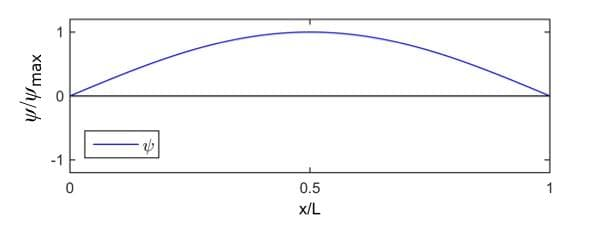
\includegraphics[width=0.7\textwidth]{bilder/Resonanz.jpg}
    \caption{Skizze zur Herleitung der Resonanz im Rohrresonator. Zu sehen ist die Grundschwingung. \cite{uni}}
\end{figure}

\subsubsection{Rohrresonator mit Blenden}
Koppelt man zwei Rohrresonatoren mit einer Blende, so verhält sich das System ähnlich zu einem 
gekoppelten Pendel. Es kommt zur einer zusätzlichen Resonanz $\omega_{R2}$ zur Ursprungsresonanz $\omega_{R1}$.
Es gilt zusätzlich $\omega_{R2}\geq \omega_{R1}$. Dies lässt sich nun durch eine Kette von Resonatoren und Blenden weitertreiben, wobei
jeweils zusätzliche Resonanzen auftreten, die im Spektrum immer dichter aneinander liegen.
Bei unendlich vielen gekoppelten Resonatoren kann man von einem Band sprechen.
Analog zu einem 1-dim-Festkörper kann man hier von einer Bandlücke sprechen.

\subsection{Analogon Teilchen im unendlichen Potenzialtopf}
Der Vergleich mit einem Teilchen im unendlichen Potenzialtopf ist dabei ein Analogon für Materie (bzw. Elektronen und Protonen)mit einem Wellencharakter, welcher durch die de-Broglie-Wellenlänge $\lambda_B$ über
\begin{equation}
    \lambda_B=\frac{h}{p}
\end{equation}
mit dem planckschen Wirkungsquantum $h$ und dem Impuls des Teilchens $p$ beschrieben werden kann.
Die Differentialgleichung für die Wellenfunktion $\Rho(x,t)$ für das Teilchen im Kasten folgt dabei aus der Schrödingergleichung
\begin{equation}
    i\hbar \frac{\partial}{\partial t}\Rho(x,t)=-\frac{\hbar^2}{2m}\frac{\partial^2}{\partial x^2}\Rho(x,t)+V(x)\Rho(x,t)
\end{equation}
mit der Teilchenmasse $m$, dem Potenzial $V(x)$. Für den unendlichen Potenzialtopf gilt $V(0 < x < L)=0$ und
$V(x \geq L)\rightarrow \infty$ und $V(x \leq 0)\rightarrow \infty$.
Damit ergibt sich die Lösung
\begin{equation}
    \Rho(x,t)=\rho(x)\cdot \exp{(-i\omega t)}
\end{equation}
und die zeitunabhängige Schrödingergleichung
\begin{equation}
    E\rho(x)=\frac{\hbar^2}{2m}\frac{\partial^2}{\partial x^2}\rho(x)
\end{equation}
mit der Energie $E$.
Für eine stehende Welle folgt daraus die Gleichung der Form
\begin{equation}
    \rho(x)=A\sin{(kx+\phi)}
    \label{eq:quant_loe}
\end{equation}
mit der komplexen Amplitude $A$, der Kreiszahl $k$ und der Phase $\phi$.
An den Rändern ergibt sich dabei eine Wellenfunktion von null, sodass aus dieser Randbedingung
$\rho(x=0)=0$ und $\rho(x=L)=0$ folgt
\begin{equation}
    k=\frac{n\pi}{L}.
    \label{eq:k}
\end{equation} 

Es wird deutlich das der Vergleich der beiden Modelle berechtigt ist. Im klassischen Fall erzeugt man eine kosinusabhängige stationäre
Druckverteilung (vgl. Gl. \ref{eq:rohr_loe}), während das quantenmechanische Modell 
eine stationäre Wahrscheinlichkeitsverteilung ergibt (vgl. Gl. \ref{eq:quant_loe}). Unterschiede zeigen sich bei den Randbedingungen.
Denn während bei dem quantenmechanischen Teilchen die Wahrscheinlichkeitsdichte verschwindet, sind an den Enden des Rohres 
die Druckunterschiede maximal, was allerdings kein Einfluss auf die erlaubten Wellenlängen hat.
Beide Modelle bilden dabei stehende Wellen für die Kreiszahl $k$ nach Gleichung \ref{eq:k} aus.


\subsection{Der Kugelresonator}
Nun wird ein Resonator mit einer Kugelform betrachtet (Hohlkugel), der aus zwei Halbkugeln besteht, welche gegeneinander verdreht werden können.
Somit können die Resonanzamplituden in Abhängigkeit des Winkels $\alpha$ gemessen werden.

Zur genauen Beschreibung des dreidimensionalen Problems der Druckverteilung wird nun die Kugelsymmetrie mit den Koordinaten des Polarwinkels $\theta$ (0 bis $\pi$)
und des Azimutwinkel $\varphi$ (0 bis $2\pi$) verwendet.
Analog zum Rohrrensonator folgt aus der Helmholtzgleichung
\begin{equation}
    \frac{\partial^2 P(\vec{r}{,}t)}{\partial t^2}=\frac{1}{\rho\kappa}\Delta P(\vec{r}{,}t)
\end{equation}
Mit dem Ansatz $P(\vec{r}{,}t)=p(\vec{r})\cos{(\omega t)}$ ergibt sich die stationäre 
Druckverteilung nach
\begin{equation}
    -\frac{w^2}{c^2}p(\vec{r})=\Delta p(\vec{r})
    \label{eq:druckverteilung_kugel}
\end{equation}
die mit dem Laplace-Operator $\Delta$ in Kugelkoordinaten zu einem Winkel- $Y_l^m(\theta{,}\varphi)$ und 
Radialanteil $f(r)$ separiert werden kann. Dabei ist $Y_l^m(\theta{,}\varphi)$ eine Kugelflächenfunktion, welche die 
stationäre, zeitunabhängige Druckverteilung beschreibt. $l$ ist die Drehimpulsquantenzahl ($0\leq l \leq n-1$),
$m$ der ganzzahlige Index mit $-l \leq m \leq l$, sodass es für jedes l nach
\begin{equation}
    Y^m_l(\theta{,}\varphi)=\sqrt{\frac{(2l+1)(l-m)!}{4\pi(l-m)!}}\cdot P_l^m(cos(\theta)) \cdot \exp({im\varphi})
\end{equation}
nicht nur eine Kugelflächenfunktion sondern $2l+1$ gibt. Somit gibt es bei einem festen $l$ für eine Kugeloberfläche
mehrere Schwingungsmöglichkeiten mit gleicher Frequenz und Energie. Man spricht von Entartung.

Setzt man den Laplace-Operator aus Gleichung \ref{eq:druckverteilung_kugel} in Kugelkoordinaten ein,
so kann die entstehende Differentzialgleichung durch den Ansatz
\begin{equation}
    p(r{,}\theta{,}\varphi)=Y_l^m(\theta{,}\varphi)\cdot f(r)
\end{equation}
in zwei Differentzialgelichung getrennt und somit gelöst werden.

\begin{table}
    \center
    \caption{Legendre-Polynome $P^m_l$ bis $l=2$}
    \begin{tabular}{c|l l l}
        & $m=0$ & $m=\pm 1$ & $m=\pm 2$ \\
        \hline
        $l=0$ & $P^0_0(\cos(\theta))=1$ & & \\
        $l=1$ & $P^0_1(\cos(\theta))=\cos(\theta))$ & $P^{\pm 1}_1(\cos(\theta))=\mp \sin(\theta)$ & \\
        $l=2$ & $P^0_2(\cos(\theta))=\frac{1}{3}(3\cos^2(\theta)-1)$ & $P^{\pm 1}_2(\cos(\theta))=\mp 3\cos(\theta)\sin(\theta)$ &$P^{\pm 2}_2(\cos(\theta))=3\sin^2(\theta)$ \\
    \end{tabular}
\end{table}

\begin{figure}
    \center
    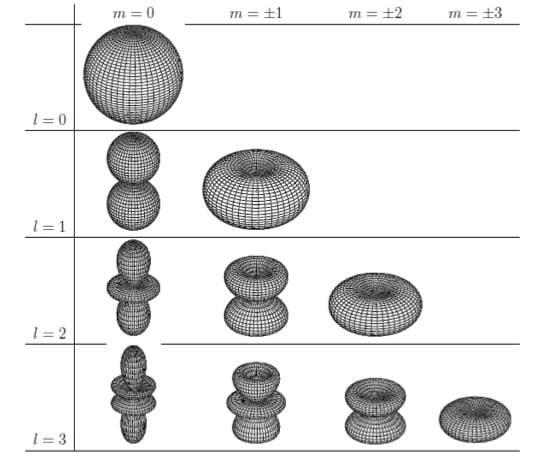
\includegraphics[width=0.7\textwidth]{bilder/schwingungsmoden.jpg}
    \caption{Betrag der Schwingungsmoden $|Y_l^m(\theta{,}\varphi|$. \cite{No}}
\end{figure}

\subsubsection*{Symmetriebrechung}
Ist die Kugelsymmetrie aufgehoben, so wird die Entartung der einzelnen m-Zustände aufgehoben, sodass die verschiedenen Kugelflächenfunktionen
zu einem $l$ nicht mehr die gleichen Energien haben. Da es zu jedem $l$ insgesamt $2l+1$ verschiedene $m$ gibt, sollte 
sich dies im Spektrum äußern. Allerdings wird im Spektrum lediglich eine Gruppe von $l+1$ Peaks deutlich, da sich die weiteren
Zustände nur in der Phase unterscheiden. Bei geringer Verformung können die Kugelflächenfunktionen näherungsweise weiterhin als Lösung angenommen werden.\\
\newline
\subsection{Analogon Wasserstoffatom}
Das Analogon zum Kugelresonator bildet das Wasserstoffatom mit einem einzigen Elektron, was ein analytisches
Lösen der Schrödingergleichung ermöglicht.
Es folgt hierfür die dreidimensionale, zeitunabhängige Schrödingergleichung
\begin{equation}
    E\psi(\vec{r})=-\frac{\hbar^2}{2m}\Delta\psi(\vec{r})+V(r)\psi(r)
\end{equation}
mit dem Coulombpotenzial $V(r)$ des Kerns. Drückt man nun die Gleichung in Kugelkoordinaten aus, 
so folgt durch einen Separationsansatz 
\begin{equation}
    \psi(r{,}\theta{,}\varphi)=Y_l^m(\theta{,}\varphi)R_{n{,}l}(r)
\end{equation}
als Lösung für die Differentialgleichung. Dabei lösen die Kugelflächenfunktionen $Y_l^m$
die rein vom Winkel abhängigen Differentialgleichungen und $R_{n{,}l}(r)$ den Radialteil. Dabei beschreibt
$n$ die Hautquantenzahl. In diesem Index unterscheidet sich das Wasserstoffatom zum Kugelresonator. Das führt dazu, dass die
die Resonanzen der beiden Systeme nicht in der gleichen Reihenfolge im Spektrum auftreten und $l$ ist dabei zu einem bestimmten
$n$ beim Kugelresonator nicht entartet, beim Wasserstoffatom jedoch schon. Grund dafür sind die verschiedenen Potenziale.

\subsection{Gekoppelte Kugelresonatoren}
Mit zwei gekoppelten Kugelresonatoren und einer Blende kann ein Wasserstoffmolekül $\text{H}_2^+$ mit einem Elektron simuliert werden.
Durch verschiedene Blenden kann eine unterschiedlich starke Kopplung dargestellt werden.
Genauso wie beim Rohrresonator mit einer Blende, bildet ich auch beim gekoppelten Kugelresonator mit Blende eine zweite Resonanz aus.
Dies lässt sich auf das Überlappen der einzelnen Atomorbitale zurückführen, die somit ein neues Molekülorbital bilden. Die Überlappung kann auf zwei Arten geschehen.
Dabei können die Vorzeichen jeweils gleich sein (Phasenverschiebung von $0°$) oder unterschiedlich (Phasenverschiebung um $180°$). Man spricht von
bindender oder antibindender Überlappung.\\

\begin{figure}
    \center
    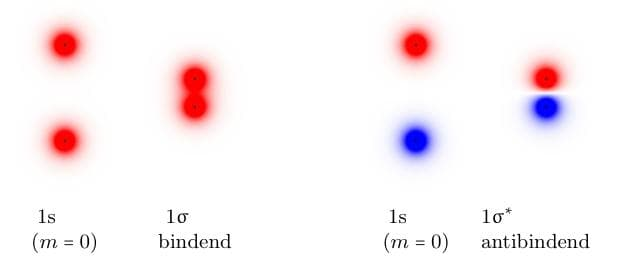
\includegraphics[width=0.7\textwidth]{bilder/mol_orbitale.jpg}
    \caption{Beispiel für bindende und antibindende Molekülorbitale beim Zusammenführen zweier Atome.
    Die Farbe spiegelt dabei die Phase wider. \cite{uni}}
\end{figure}
Zwei Atome mit 1s-Orbitalen bilden somit bei positivem Vorzeichnen ein zugehöriges 1$\sigma$-Molekülorbital. Die neun Orbitale werden dabei mit
griechischen Buchstaben gekennzeichnet und resultieren aus der magnetischen Quantenzahl $m$. Aus $m=0$ folgt somit die neue Orbitalbezeichnung 
$\sigma$, $m=1$ fürt zu einen $\pi$-Orbital.
Die Hautquantenzahl unterscheidet dabei die Orbitale gleicher Symmetrien aber unterschiedlichen Energien.
Zusatzlich kann die Wahrscheinlichkeit der Lage des Elektrons beschrieben werden. Dabei hat das 1$\sigma$ Molekülorbital eine hohe Wahrscheinlichkeit für die Lage zwischen
den beiden Atomkernen (bindender Zustand, energetische tiefere Lage). Bei niedriger Auftrittswahrscheinlichkeit beim
antibinden Zustand 1$\sigma^*$ liegt der Zustand energetisch höher als der Zustand des Atoms.









